\documentclass[12pt]{extarticle}
\usepackage{alphabeta}
\usepackage{graphicx}
\usepackage{amssymb,amsthm,amsmath, xcolor}
\usepackage{listings, multicol}
\usepackage{hyperref}

\begin{document}
\begin{center}
\textbf{Airline Traffic Optimization} \\
\begin{center}
Carter Glazer, Jiajun Chen, Satvik Kannekanti
\end{center}
\end{center}

\section*{\small Motivation:}
\hspace{1cm}
Our motivation to develop an MILP model to optimize flight routing stemmed from Jiajun, an international student, and Carter, from Los Angeles, who often faced flight delays and noticed inefficiencies in air traffic management.
\section*{\small Problem:}
\hspace{1cm}
An airline has 4 planes all starting at Los Angeles International Airport (LAX). We want to optimize the minimum total distance for the daily flight routing for the 4 planes. The planes must schedule flights to 13 other major airports: Hartsfield-Jackson Atlanta International Airport (ATL), San Francisco (SFO), New York (JFK), Denver (DEN), Dallas/Fort Worth (DFW), Chicago O'Hare (ORD), Detroit Metropolitan (DTW), Orlando (MCO), Las Vegas (LAS), Seattle (SEA), Phoenix (PHX), Minneapolis/St. Paul (MSP), and Boston (BOS). Each airport must be visited exactly once per day by one of the four planes. Furthermore, at the end of the day, the planes must return to the starting airport. Lastly, each plane must fly either 4 or 5 flights each day.

\section*{\small Objective:}
\hspace{1cm} The objective will be to minimize the total distance flown across the four planes.

\section*{\small Data:}
The data was data for flight distances came from \href{https://www.airmilescalculator.com/
}{here}

\section*{\small Variables:}
Let n be the number of airports, so in this case, let n = 14. \\ \\
Airports = \{LAX, ATL, SFO, JFK, DEN, DFW, ORD, DTW, MCO, LAS, SEA, PHX, MSP, BOS\} \\
We will assign each airport a number, so airports = \{1, 2, 3, 4, 5, 6, 7, 8, 9, 10, 11, 12, 13, 14\} \\
The starting airport, LAX, is 1. \\ \\
Let w, x, y, z represent the four planes \\
Let $w_{i,j}$ = 1 if plane 1 travels from airport i to airport j, 0 otherwise. \\
Let $x_{i,j}$ = 1 if plane 1 travels from airport i to airport j, 0 otherwise. \\
Let $y_{i,j}$ = 1 if plane 1 travels from airport i to airport j, 0 otherwise. \\
Let $z_{i,j}$ = 1 if plane 1 travels from airport i to airport j, 0 otherwise. \\
Let $d_{i,j}$ be the distance from airport i to airport j. \\ \\
Let t be variable to avoid subtours. \\
Here is the code for the variables: \\ \\
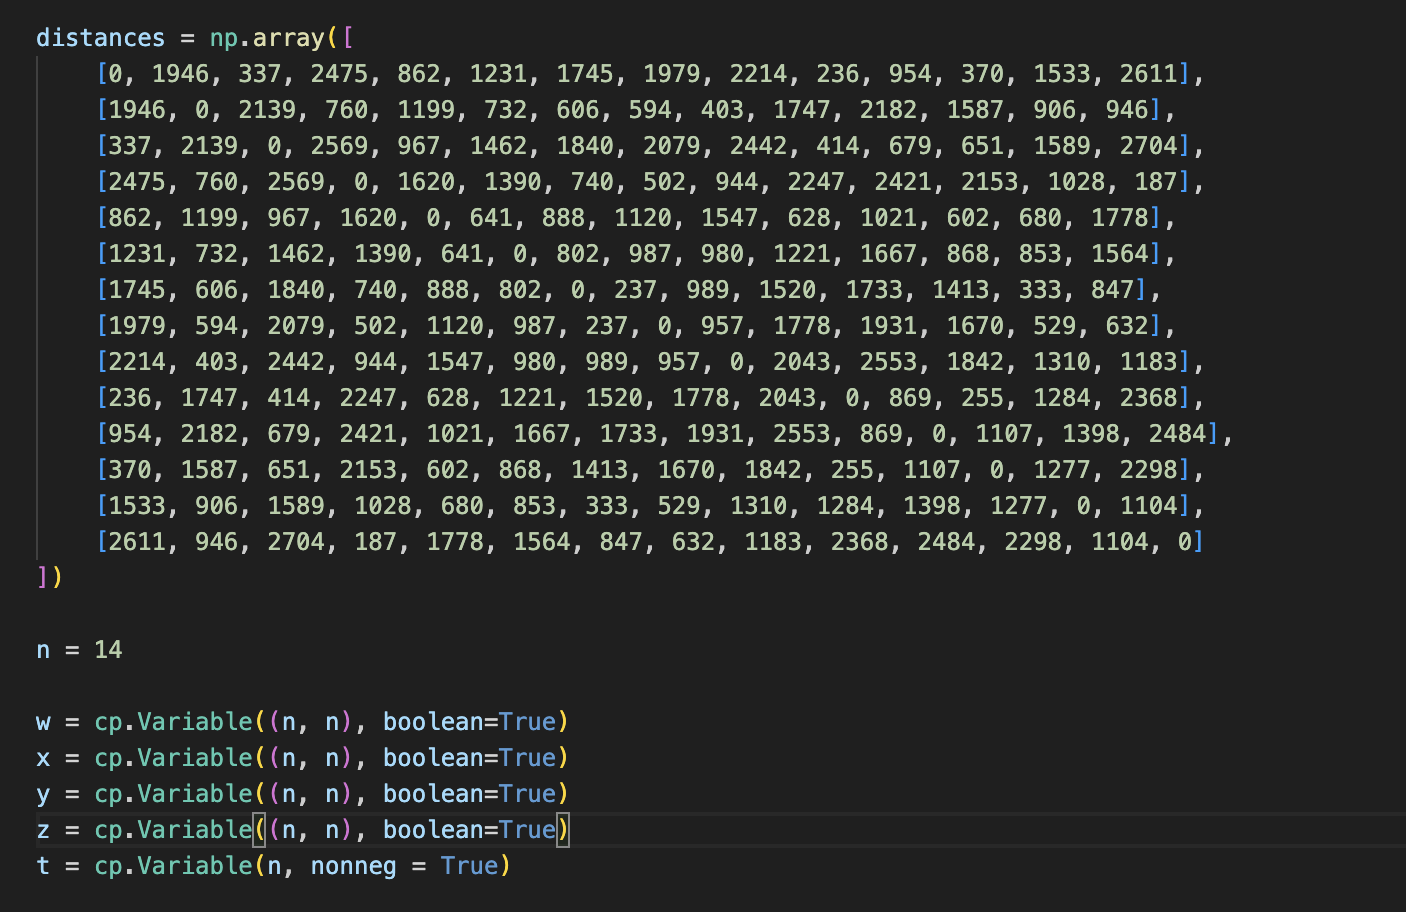
\includegraphics[scale = .5]{images/OptVars.png}

\section*{\small Objective Function:}
The objective function will be the distance matrix multiplied by the sum of the plane matrices. \\
Written Mathematically as:
\begin{align*}
\sum_{i=1}^n\sum_{j=1}^nd_{i,j}(w_{i,j} + x_{i,j} + y_{i,j} + z_{i,j})
\end{align*}
With the code: \\ \\
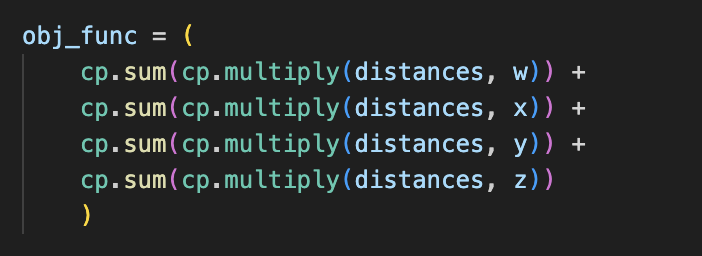
\includegraphics[scale = .5]{images/ObjFunc.png}
\section*{\small Constraints:}
The first constraint are that each airport (aside from the starting airport) must be departed from and arrived at exactly once between all 4 planes.
\begin{align*}
&\text{For all } i > 1 \text{ (without starting airport):} \\
&\hspace{1.5cm}\sum_{j=2}^n w_{i,j} + x_{i,j} + y_{i,j} + z_{i,j} = 1 \\
&\text{For all } j > 1 \text{(without starting airport):} \\
&\hspace{1.5cm}\sum_{i=2}^n w_{i,j} + x_{i,j} + y_{i,j} + z_{i,j} = 1 \\
\end{align*}
The corresponding code: \\ \\
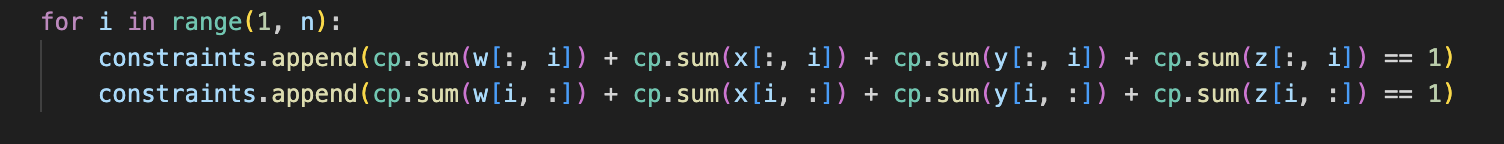
\includegraphics[scale = .5]{images/constraints1.png} \\

The next constraint is to ensure that no flight departs and arrives at the same airport.
\begin{align*}
&\sum_{i=1}^nw_{i,i} = 0 \\
&\sum_{i=1}^nx_{i,i} = 0 \\
&\sum_{i=1}^ny_{i,i} = 0 \\
&\sum_{i=1}^nz_{i,i} = 0 \\
\end{align*}
The corresponding code: \\ \\
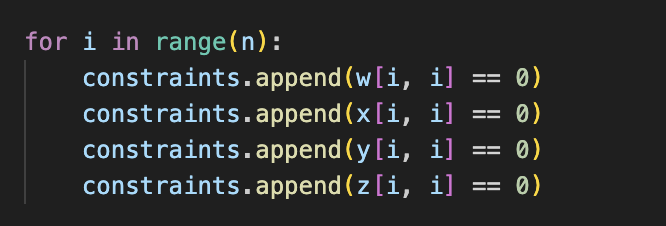
\includegraphics[scale = .5]{images/constraints2.png} \\

The next constraint is to ensure that the number of flights arriving to each airport is the same as the number of flights departing from each airport.
\begin{align*}
&\text{For all } i \text{:} \\
&\hspace{1.5cm}\sum_{j=1}^nw_{i,j} = \sum_{j=1}^nw_{j,i} \\
&\hspace{1.5cm}\sum_{j=1}^nx_{i,j} = \sum_{j=1}^xw_{j,i} \\
&\hspace{1.5cm}\sum_{j=1}^ny_{i,j} = \sum_{j=1}^ny_{j,i} \\
&\hspace{1.5cm}\sum_{j=1}^nz_{i,j} = \sum_{j=1}^nz_{j,i} \\
\end{align*}
The corresponding code: \\ \\
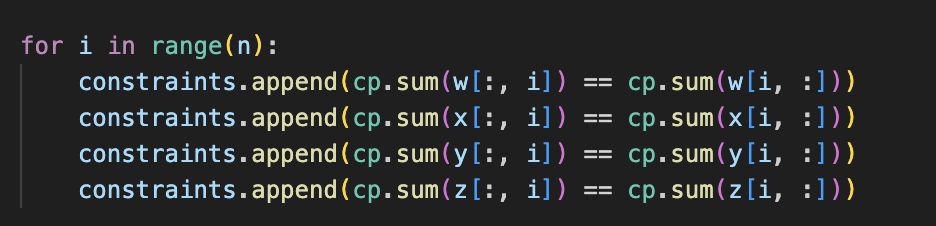
\includegraphics[scale = .5]{images/constraints3.png} \\

The next constraint is the number of flights constraint. Each plane must fly either 4 or 5 flights
\begin{align*}
&4 \leq\sum_{i=1}^n\sum_{j=1}^nw_{i,j} \leq 5 \\
&4 \leq\sum_{i=1}^n\sum_{j=1}^nx_{i,j} \leq 5 \\
&4 \leq\sum_{i=1}^n\sum_{j=1}^ny_{i,j} \leq 5 \\
&4 \leq\sum_{i=1}^n\sum_{j=1}^nz_{i,j} \leq 5 \\
\end{align*}
Here is the code for those constraints: \\ \\
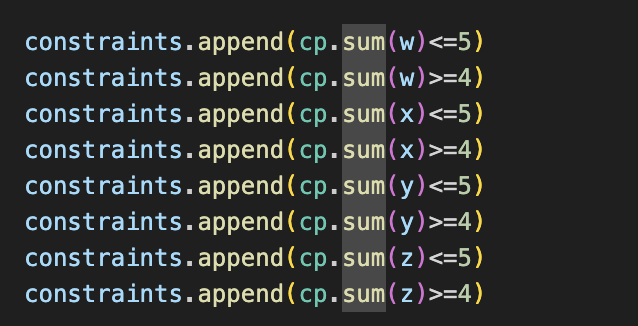
\includegraphics[scale = .5]{images/constraints4.png} \\

The next constraint is the starting airport constraint.
\begin{align*}
&\sum_{j=2}^nw_{i,j} = 1 \\
&\sum_{j=2}^nx_{i,j} = 1 \\
&\sum_{j=2}^ny_{i,j} = 1 \\
&\sum_{j=2}^nz_{i,j} = 1 \\
\end{align*}
Since the number of incoming flights must be equal to the number of departing flights (specified earlier), this ensures at some point, each plane will return to the starting airport. \\ \\
Here is the corresponding code:\\ \\
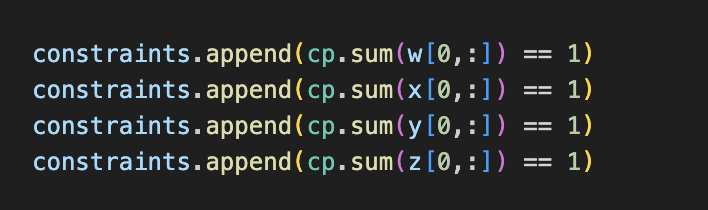
\includegraphics[scale = .5]{images/constraints5.png} \\

The final constraint is too eliminate sub tours. I used the same idea with the variable t as used in class.
\begin{align*}
&\text{For all } 2 \leq i, j \leq n \text{, and i does not equal j:} \\
&\hspace{1.5cm}t_i - t_j + (n-1)w_{i,j} \leq n-2 \\
&\hspace{1.5cm}t_i - t_j + (n-1)x_{i,j} \leq n-2 \\
&\hspace{1.5cm}t_i - t_j + (n-1)y_{i,j} \leq n-2 \\
&\hspace{1.5cm}t_i - t_j + (n-1)z_{i,j} \leq n-2 \\
\end{align*}
The corresponding code: \\ \\
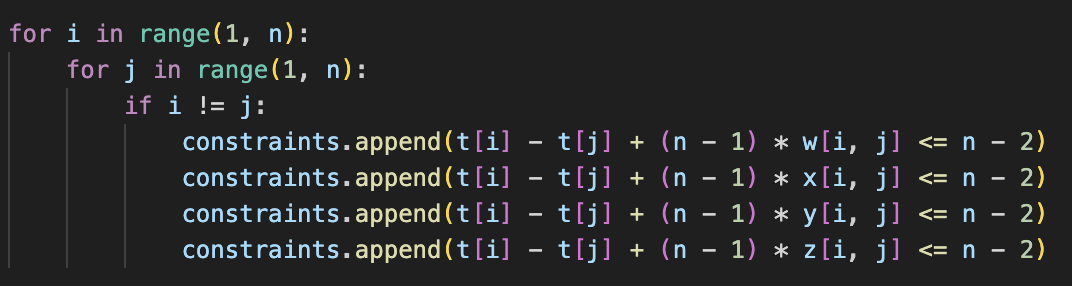
\includegraphics[scale = .5]{images/constraints6.png} \\

\section*{\small Running the code:}
We ran the code as follows. \\ \\
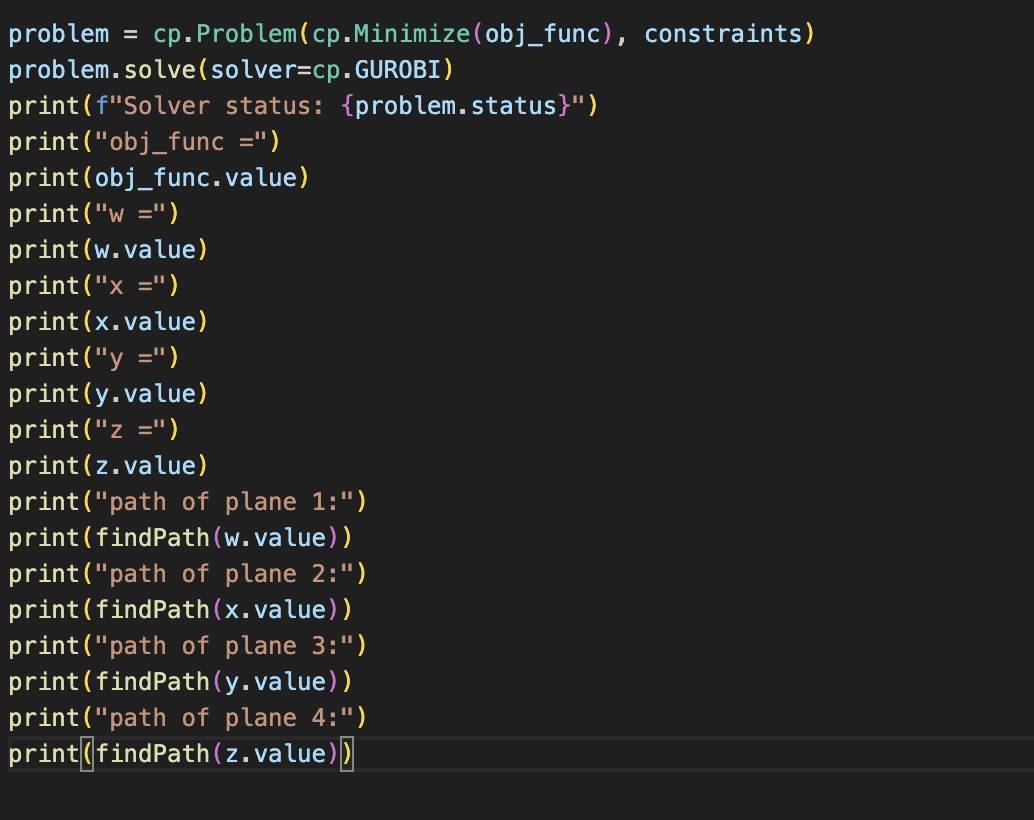
\includegraphics[scale = .5]{images/runningCode.png} \\ \\
The findPath function prints out the path of the plane that calls it. \\
Here is the code for it: \\ \\
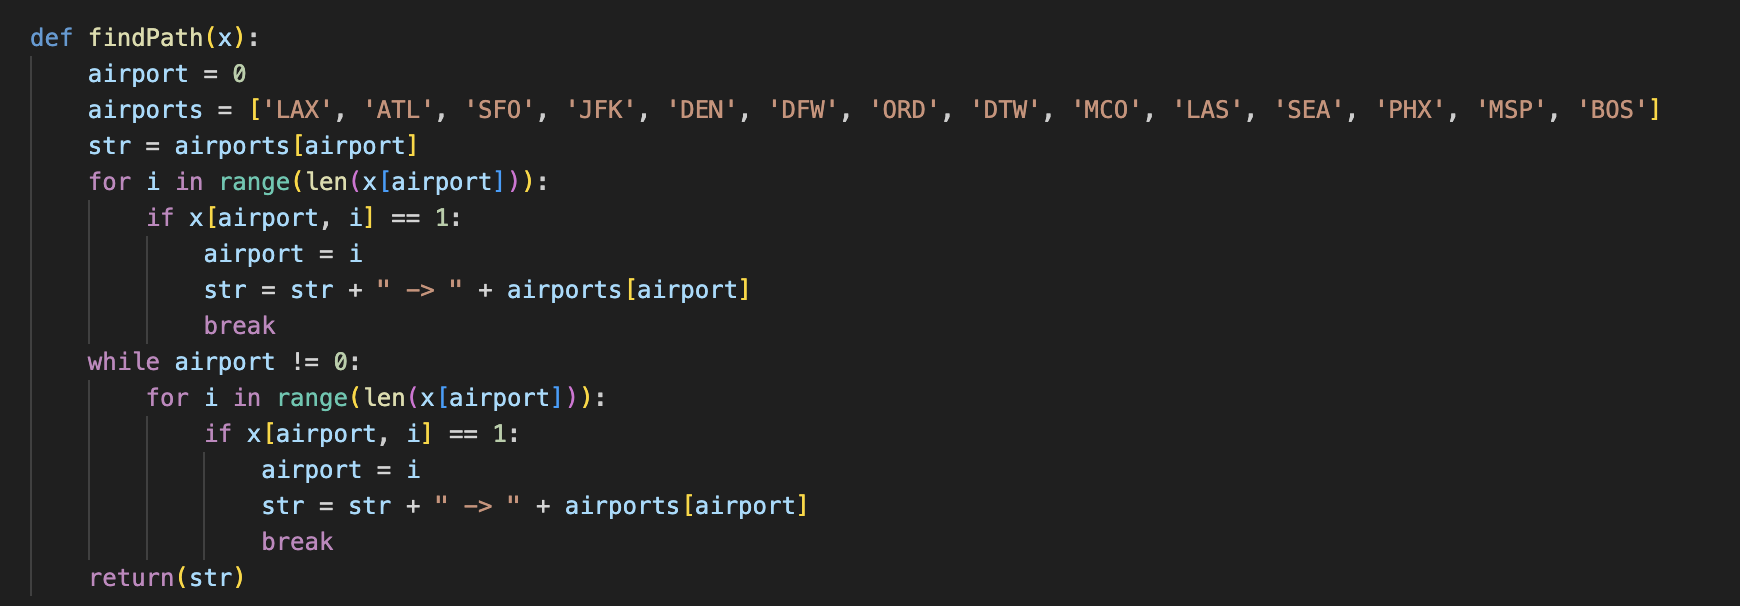
\includegraphics[scale = 0.5]{images/findPath.png} \\

\section*{\small Results:}
After running the code, we got an optimal value of 14997.0 miles. \\
The flight paths of the 4 planes are as follows: \\ \\
Plane w (plane 1): \\
LAX -$>$ BOS -$>$ JFK -$>$ MCO -$>$ ATL -$>$ LAX \\ \\
Plane x (plane 2): \\
LAX -$>$ MSP -$>$ DTW -$>$ ORD -$>$ LAX \\ \\
Plane y (plane 3): \\
LAX -$>$ DEN -$>$ DFW -$>$ PHX -$>$ LAX \\ \\
Plane z (plane 4): \\
LAX -$>$ SFO -$>$ SEA -$>$ LAS -$>$ LAX \\ \\

Additionally, here is the objective value, objective matrices, and paths as outputted by the code: \\ \\
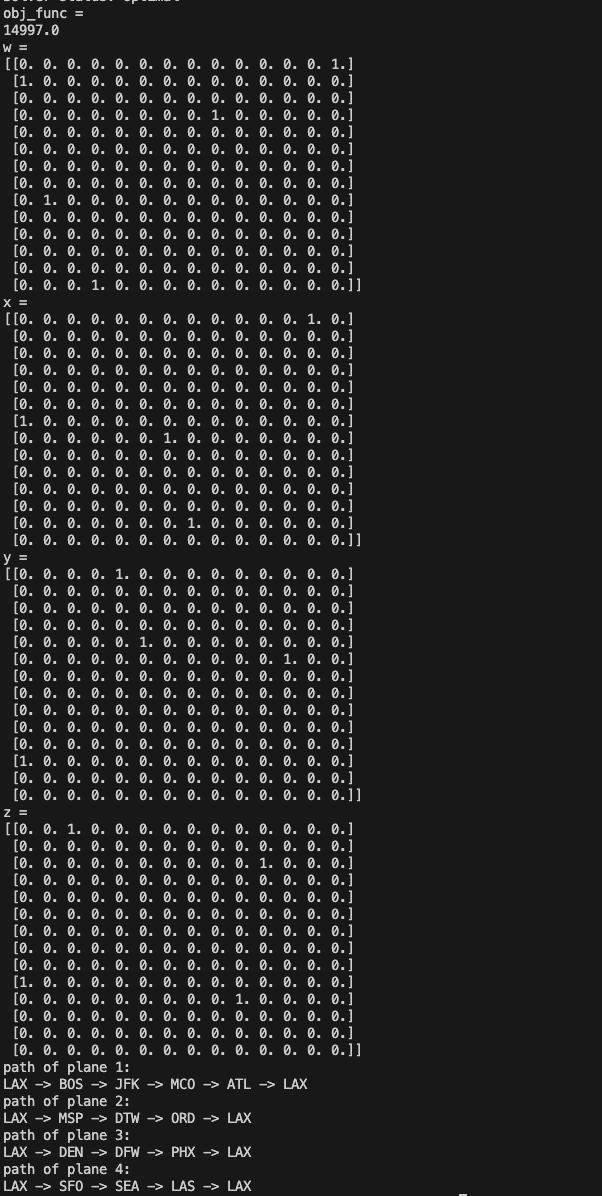
\includegraphics[scale = 0.5]{images/output.png} \\
As mentioned in the definition of the binary variables, if $w_{i,j}$ (w[i, j]) = 1 that means plane w has a flight from airport i to airport j. \\

\newpage
\section*{\small Appendix:}
\begin{align*}
&\text{\href{https://github.com/glazer77/ISE-3230-Project}{Github Repository}} \\
&\text{\href{https://github.com/glazer77/ISE-3230-Project/raw/refs/heads/main/optimizationVideo.mp4}{Video}} \\
\end{align*}
The optimization aprt of the code was written by everyone, the findPath was written by Carter. The formulation was done by everyone. The making of the latex document and pdf output was done by Carter. The final presentation was made by Satvik and Jiajun.
\end{document}



